\documentclass[11pt]{article}

% =============================
% Packages
% =============================
\usepackage[margin=1in]{geometry}
\usepackage{graphicx}
\usepackage{amsmath, amssymb}
\usepackage{siunitx}
\usepackage{booktabs}
\usepackage{caption}
\usepackage{subcaption}
\usepackage{float}
\usepackage{hyperref}
\usepackage{cite}
\usepackage{xcolor}
\usepackage{enumitem}
\usepackage{tikz}
\usetikzlibrary{shapes.geometric, positioning}
\usepackage[europeanresistors, americaninductors, siunitx]{circuitikz}

% =============================
% Custom Commands
% =============================
\newcommand{\vect}[1]{\mathbf{#1}}

% =============================
% Title Information
% =============================
\title{\textbf{Differential Probe V1}\\
\large Madrigal Technologies}

\author{Ricardo Ramirez}
%Department or Affiliation}

\date{\today}

\begin{document}

\maketitle

\begin{abstract}
\noindent f
\end{abstract}

\section{Introduction}
Provide background, motivation, and the goal of the project. Clearly state what problem you are addressing and why it matters.


\section{Requirements}

\begin{enumerate}
	\item \textbf{Measurement Capabilities} 
	\begin{itemize}
		\item \textbf{Input Voltage} 
			\begin{itemize}
				\item \textbf{+/- 50V}
			\end{itemize}
		\item \textbf{Attenuation}
			\begin{itemize}
				\item \textbf{10x}
			\end{itemize}
		\item \textbf{AC Measurements}
			\begin{itemize}
				\item Not Included in v1 (planned for later version)
			\end{itemize}
	\end{itemize}

\end{enumerate}

\section{Theory / Background}

Differential probes are needed when we need to measure the difference between two nodes. It is possible to make differential measurements using two oscilloscope probes by connecting the grounds together and placing the probe at each voltage point and then using the math function on the oscilloscope to subtract the voltages from each other. This method has its limitations and is only viable for low frequency signals and can introduce measurement errors due to mismatched probe characteristics.

\begin{figure}[h] % 'h' means "here"
    \centering
    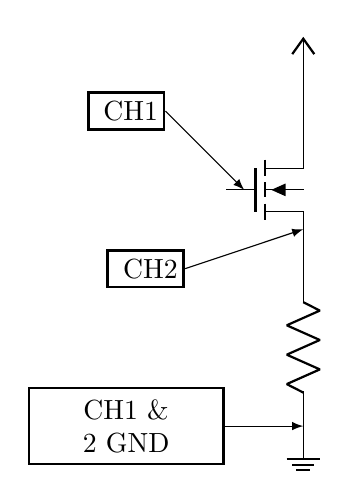
\begin{tikzpicture}
	% Paths, nodes and wires:
	\node[nfet] at (8, 6){};
	\draw (8, 5) to[american resistor] (8, 3);
	\draw (8, 5) |- (8, 5.23);
	\node[ground] at (8, 3){};
	\draw[-latex] (6.25, 7) -- (7.25, 6);
	\draw[-latex] (6.5, 5) -- (8, 5.5);
	\node[shape=rectangle, draw, line width=1pt, minimum width=0.965cm, minimum height=0.465cm] at (5.75, 7){} node[anchor=center, align=center, text width=0.577cm, inner sep=6pt] at (5.75, 7){CH1};
	\node[shape=rectangle, draw, line width=1pt, minimum width=0.965cm, minimum height=0.465cm] at (6, 5){} node[anchor=center, align=center, text width=0.577cm, inner sep=6pt] at (6, 5){CH2};
	\draw[-latex] (7, 3) -- (8, 3);
	\node[shape=rectangle, draw, line width=1pt, minimum width=2.465cm, minimum height=0.965cm] at (5.75, 3){} node[anchor=center, align=center, text width=2.077cm, inner sep=6pt] at (5.75, 3){CH1 \& 2 GND};
	\node[vcc] at (8, 7.5){};
	\draw (8, 7.5) |- (8, 6.77);
\end{tikzpicture}
    \caption{Subtraction Probe Method}
    \label{fig:SUB}
\end{figure}


Ground reference is not available on all power-conversion devices, and thus, these measurements need to be made using differential probes. For example, consider the following measurements: inductor and transformer voltages, drain to source voltage on a MOSFET, and voltage drops on ungrounded resistors. 

\vspace{1em}

\noindent The best way to make these measurements is by using a dedicated differential probe (simple circuit shown in Figure 1). This type of probe uses a differential amplifier to generate an output of the difference of the two input signals. Unlike the previous method that uses up two oscilloscope channels, this probe only requires one as it handles the operation it self. 

\vspace{1em}

\noindent Compared to the subtractive method, active differential probes have a wider bandwidth range and small input capacitance. 

\begin{figure}[h] % 'h' means "here"
    \centering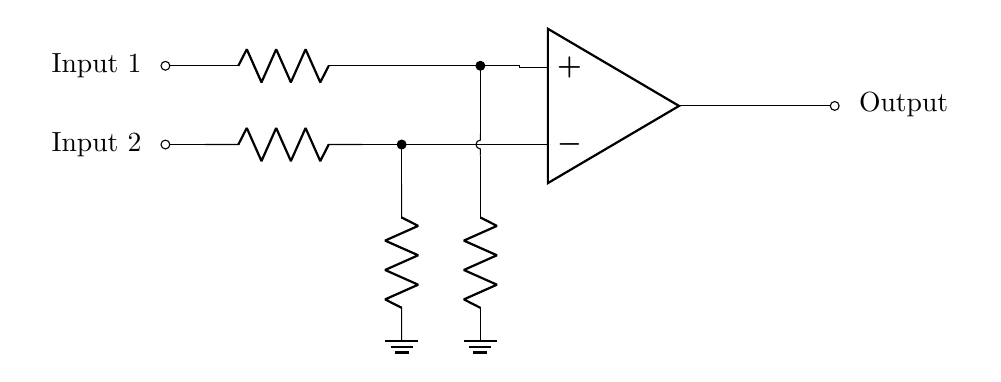
\begin{tikzpicture}
	% Paths, nodes and wires:
	\node[op amp, yscale=-1] at (9.19, 5.49){};
	\draw (4, 6) to[american resistor] (6, 6);
	\draw (4, 5) to[american resistor] (6, 5);
	\draw (6.5, 4.5) to[american resistor] (6.5, 2.5);
	\draw (7.5, 4.5) to[american resistor] (7.5, 2.5);
	\draw (6, 6) -| (8, 5.98);
	\draw (6.5, 4.5) -| (6.5, 5);
	\node[jump crossing, rotate=90] at (7.5, 5){};
	\draw (7.5, 5.14) -| (7.5, 6);
	\draw (6, 5) -- (7.14, 5);
	\draw (7.14, 5) -- (8, 5);
	\draw (7.5, 4.86) -| (7.5, 4.5);
	\node[circ] at (7.5, 6){};
	\node[circ] at (6.5, 5){};
	\node[tlground] at (6.5, 2.5){};
	\node[tlground] at (7.5, 2.5){};
	\draw (3.5, 6) -- (4, 6);
	\draw (3.5, 5) -- (4, 5);
	\node[ocirc] at (3.5, 6){};
	\node[ocirc] at (3.5, 5){};
	\node[shape=rectangle, minimum width=1.715cm, minimum height=0.965cm] at (2.625, 6){} node[anchor=center, align=center, text width=1.327cm, inner sep=6pt] at (2.625, 6){Input 1};
	\node[shape=rectangle, minimum width=1.715cm, minimum height=0.965cm] at (2.625, 5){} node[anchor=center, align=center, text width=1.327cm, inner sep=6pt] at (2.625, 5){Input 2};
	\draw (10.38, 5.49) -| (12, 5.5);
	\node[ocirc] at (12, 5.49){};
	\node[shape=rectangle, minimum width=1.715cm, minimum height=0.965cm] at (12.875, 5.5){} node[anchor=center, align=center, text width=1.327cm, inner sep=6pt] at (12.875, 5.5){Output};
\end{tikzpicture}
    \caption{Differential Probe Circuit Diagram}
    \label{fig:opamp}
\end{figure}

\subsection{Input Stage}
\noindent  

\subsection{Amplifier Stage}

\subsection{Output Stage}

\noindent The output of an ideal differential amplifier is given by:
\begin{equation}
V_{out} = A_d(V_+ - V_-)
\end{equation}
Where $A_d$ is the differential gain.
\section{System Design / Methodology}
Describe the overall approach. This can be broken into subsections.

\subsection{Block Diagram} % Created using CircuitTikZ Designer


\subsection{Input Protection}
\noindent 
 



\subsection{Hardware Design}
Describe schematics, components, and design choices.

\subsection{Software / Firmware}
Describe algorithms, control logic, or firmware structure.

\section{Experimental Setup}
Explain how the system was tested, including equipment, configurations, and procedures.

\section{Results}
Present measured or simulated results. Use figures and tables where appropriate.


\end{document}